\documentclass[10pt,twocolumn,letterpaper]{article}

\usepackage{cvpr}
\usepackage{times}
\usepackage{epsfig}
\usepackage{graphicx}
\usepackage{amsmath}
\usepackage{amssymb}

% Include other packages here, before hyperref.

% If you comment hyperref and then uncomment it, you should delete
% egpaper.aux before re-running latex.  (Or just hit 'q' on the first latex
% run, let it finish, and you should be clear).
\usepackage[breaklinks=true,bookmarks=false]{hyperref}

\cvprfinalcopy % *** Uncomment this line for the final submission

\def\cvprPaperID{****} % *** Enter the CVPR Paper ID here
\def\httilde{\mbox{\tt\raisebox{-.5ex}{\symbol{126}}}}

% Pages are numbered in submission mode, and unnumbered in camera-ready
%\ifcvprfinal\pagestyle{empty}\fi
\setcounter{page}{1}
\begin{document}

%%%%%%%%% TITLE
\title{Helping the Color Blind See Color}

\author{Carolyn Chen\\
Princeton University\\
Princeton, NJ\\
{\tt\small clc4@princeton.edu}
% For a paper whose authors are all at the same institution,
% omit the following lines up until the closing ``}''.
% Additional authors and addresses can be added with ``\and'',
% just like the second author.
% To save space, use either the email address or home page, not both
\and
Dorothy Chen\\
Princeton University\\
Princeton, NJ\\
{\tt\small dschen@princeton.edu}
}

\maketitle
%\thispagestyle{empty}

%%%%%%%%% ABSTRACT
\begin{abstract}
   In this paper we propose our final project for our Computer Vision class, COS 429, taught by Professor Xiao. We begin by discussing the motivation behind the research problem and why it is a relevant topic, followed by a brief survey of existing research on this topic. We then suggest a possible procedure to implement the algorithm and end with a discussion on how we will measure the success of our project. 
\end{abstract}

%%%%%%%%% BODY TEXT
\section{Motivation}

We want to implement an algorithm that can re-color images to make them more accessible for people with color vision deficiency (CVD). This is an important topic to consider because genetic photoreceptor disorders are the most common cause of CVD, manifesting in 8\% of Caucasian males, 5\% of Asiatic males, and 3\% of African-American and Native-American males [4]. Details that are easily seen by people with normal color vision may be completely overlooked by people with CVD due to differences in color perception. Furthermore, there are different types of CVD, and people with CVD tend to have different scales of the condition. This shows that there must be a way to adapt the algorithm based on the severity of CVD for a unique user. Thus, we hope to accomplish this goal by providing an adaptable algorithm that uses calibration to modify certain parts of an image to make them more visible to people with CVD. 

%------------------------------------------------------------------------
\section{Existing Research}

There has already been some extensive research on this topic. Below we summarize a sample of papers we are using to help us with this project.

%-------------------------------------------------------------------------
\subsection{"Adapting Palettes to Color Vision Deficiencies by Genetic Algorithm"}

The authors discuss a method to choose a color palette that will optimize the balance between aesthetics and accessibility requirements for people with CVD. While this is mainly aimed toward assisting user interface designers in picking appropriate color palettes, its discussion on how they choose the color palette may very well come in handy for our own algorithm, when we need to choose an appropriate manner by which to manipulate the image. 


%-------------------------------------------------------------------------
\subsection{"Image Recolorization for the Colorblind"}

The authors propose a re-coloring algorithm that is completely automatic, using a four step procedure that involves a transformation into a different color space, clustering via Gaussian Mixture Modeling, an optimization procedure that focuses on changing the colors that are perceived differently by people with CVD, and finally a Gaussian mapping for interpolation for re-coloring. Basically, this re-coloring algorithm finds an optimal mapping to maintain the contrast between pairs of “key” colors.

%-------------------------------------------------------------------------
\subsection{"An Efficient Naturalness-Preserving Image-Recoloring Method for Dichromats"}

The authors present a different algorithm that runs through similar major steps, here described as image quantization, mass-spring optimization, and reconstruction. The major differences between this paper and the previous one is that this one models the recoloring approach as a mass-spring system, which supposedly “lends itself to an efficient GPU implementation.” Furthermore, the authors emphasize that their implemented technique highlights visual details, preserving as much as the image’s original colors as possible. This method is again an automatic algorithm, meaning it does not take in any parameters that are user defined.

%-------------------------------------------------------------------------
\subsection{"An Interface to Support Color Blind Computer Users"}

This paper presents a different approach by implementing a user-adaptable algorithm, as opposed to an automatic method as described above. While there are reasonable concerns with why researchers stray from user-assisted methods, for they may make the results highly dependent on user-defined parameters and may cause unrealistic results, we think that it may be worth combining this paper’s idea of supporting personalization or adaptability to an algorithm as described in the second or third paper, due to the above mentioned concern of different scales of color-blindness. 


%-------------------------------------------------------------------------
\section{Methodology}

Similar to the above papers, we plan to break this problem up into the following parts.

%-------------------------------------------------------------------------
\subsection{Calibration}

We would like our algorithm to be adaptable to a specific user’s severity of color-blindness, for different people have different types of CVD and therefore different perceptions of color. Consequently, this algorithm would be user-assisted rather than automatic. As previously discussed, there are pros and cons to implementing a user-assisted algorithm, but perhaps it may also result in a more accurate re-colored image tailored to the person. An idea of how we would calibrate this would be by allowing users to manipulate some images with a simple interface until they can see the content (perhaps we will let them manipulate a couple Isihara test plates). 

%-------------------------------------------------------------------------
\subsection{Image quantization}

Based on the above results, we will extract relevant parameters that will allow us to calculate a new map of colors, similar to how the two papers above “quantize” or “cluster” the colors in the image. We will base this algorithm off of that described in [2], except instead of hardcoding the different color gamut parameters for different conditions, we will use the parameters extracted from the calibration step.

%-------------------------------------------------------------------------
\subsection{Optimization}

This part of the algorithm will perform the optimization step, which will minimize the difference between the perceived image and the manipulated image, only to create a sufficient contrast to allow for visibility of the content. We will use the two papers above as starting points for this part of the algorithm. 

%-------------------------------------------------------------------------
\subsection{Re-coloring}

This step is also described in the papers, which we will implement. 

%-------------------------------------------------------------------------
\subsection{Stretch goal 1}

The above papers all manipulate the images on a global scale, meaning that the re-coloring is performed on the entire image when, perhaps, it may not be necessary. [3] stresses the importance of preserving naturalness, and perhaps this may also mean preserving as much of the original image as possible. Therefore, we propose that if the above is implemented to a reasonable degree, we will try to further our algorithm to only manipulate certain areas that may be a cause of confusion for the person. A possible way to implement this would be to use the calibration results to generate a couple patches to slide along the image and check whether or not the histogram of gradients is similar or not. Once a patch of the image is found, we would propagate the re-coloring from that point, so as to avoid unnecessary re-coloring of the whole image.

%-------------------------------------------------------------------------
\subsection{Stretch goal 2}

To simulate real-time manipulation, we will try to re-color videos. This would involve some algorithm like Lucas-Kanade to track the relevant patches to manipulate rather than recalculating all the values for every frame. 

%------------------------------------------------------------------------
\section{Evaluation Metrics}

To simulate what the images look like to a person with CVD, we will use the algorithm described in [4]. In order to measure the success of our project, we will set a requirement that our output will look at least as good as the results depicted in [2] and [3]. Meaning, if the output is similar to the output of the existing algorithms, then we will be satisfied. One way we could do this is to find the contrast between portions of the image. Ideally, we would want the contrast values of the processed image (from the viewpoint of someone with CVD) to be similar to those of the original image to someone with normal vision. This would mean that people with CVD are able to distinguish regions with different colors that they were not able to before. 

An example of the original image and processed outputs can be found in figure \ref{fig:flowers}. If our algorithm is better, as in it exhibits more preservation of the original image while still providing new contrast for a person with CVD, then we will be even happier. Further, to obtain more quantitative results, we may ask for volunteers with CVD to try out our algorithm and test how many Ishihara test plates they can identify after calibration and re-coloring. Finally, to see how our algorithm does on ``real-world'' data, we may ask the same volunteers to examine images that typically give individuals with CVD trouble and see how calibration and re-coloring may improve performance. 

\begin{figure}[h]
  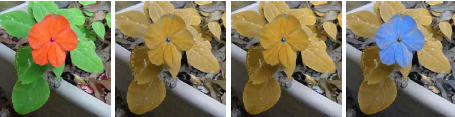
\includegraphics[width=0.5\textwidth]{flowers.png}
  \caption{(a) is with regular vision; (b) is a simulation of a person with CVD's view; (c) is an intermediate step in algorithm described in [3]; (d) is an example of a processed image}
  \label{fig:flowers}
\end{figure}

%------------------------------------------------------------------------
\section{References}

{\small
\bibliographystyle{ieee}
\bibliography{egbib}
[1] Troiano, Luigi, Cosimo Birtolo, and Maria MIranda. "Adapting Palettes to Color Vision Deficiencies by Genetic Algorithm." ACM, 2008 Web. 30 Nov. 2014.

[2] Huang, Jia-Bin, Chu-Song Chen, Tzu-Cheng Jen, and Sheng-Jyh Wang. "Image Recolorization for the Colorblind." National Science Council of Taiwan, 2009. Web. 30 Nov. 2014.

[3] Kuhn, Giovane R., Manuel M. Oliveira, and Leandro A. Fernandez. "An Efficient Naturalness-Preserving Image-Recoloring Method for Dichromats." Instituto De Informática, 19 Oct. 2008. Web. 30 Nov. 2014.

[4] Jefferson, Luke, and Richard Harvey. "An Interface to Support Color Blind Computer Users." ACM, 2007. Web. 30 Nov. 2014.

}

\end{document}
